Once the marginal temporal structure of the two price series has been established, the
natural next step is to move beyond average dynamics and focus on the tails of the
distribution. In this section we therefore study the distributional behaviour of extreme
observations in both the upper tail (very high prices) and the lower tail (mainly negative
prices) using the Peaks-over-Threshold (POT) framework from Extreme Value Theory (EVT).

The section is organised as follows. We first recall the theoretical foundations of the
POT method and the Generalised Pareto Distribution (GPD). We then carry out the threshold
selection, the GPD estimation and the goodness-of-fit diagnostics separately for the upper
and lower tails of the French and German series. We complement the maximum-likelihood
estimates with the semi-parametric Hill estimator. Finally, we draw the implications of this analysis for the subsequent
copula and Hawkes sections.

% ------------------------------------------------------------
\subsection{The Peaks-over-Threshold Framework}
\label{subsec:pot_theory}
% ------------------------------------------------------------

The Peaks-over-Threshold method rests on the
\textbf{Pickands–Balkema–de Haan theorem}, which states that, for a sufficiently high
threshold $u$, the conditional distribution of the exceedances

\begin{equation}
    Y = X - u \quad \text{for } X > u
    \label{eq:upper_excess}
\end{equation}

converges to a \textbf{Generalised Pareto Distribution (GPD)}:

\begin{equation}
    F_{\xi,\beta}(y) = 1 - \left(1 + \frac{\xi\, y}{\beta}\right)^{-1/\xi},
    \quad y > 0, \quad \beta > 0,
    \label{eq:gpd_upper}
\end{equation}

where $\xi \in \mathbb{R}$ is the \emph{shape} parameter and $\beta > 0$ is the
\emph{scale} parameter. The sign of $\xi$ determines the tail regime:
$\xi > 0$ corresponds to a heavy-tailed (Fréchet) distribution with a polynomial
decay; $\xi = 0$ corresponds to an exponential tail (Gumbel); and $\xi < 0$
corresponds to a bounded upper tail (Weibull).

A key diagnostic tool for threshold selection is the \textbf{Mean Excess Plot (MEP)}, which traces the empirical mean excess function
$
e(u') = E[X - u' \mid X > u']
$
as a function of the threshold \(u'\). Under the GPD model, \(e(u')\) is approximately linear 
for sufficiently high thresholds. In practice, we select a threshold in the region where the MEP exhibits 
approximate linearity: this corresponds to a value of \(u'\) large enough that the GPD provides a reasonable 
approximation, while retaining enough exceedances for reliable estimation.

\paragraph{Lower-tail exceedances.}
The same framework applies to the lower tail via the standard reflection trick. For a
low threshold $u$, the \emph{lower exceedances} (or deficits) are defined as

\begin{equation}
    Y = u - X \quad \text{for } X < u,
    \label{eq:lower_excess}
\end{equation}

which is equivalent to applying the POT method to the mirrored series $-X$.

\paragraph{Maximum-likelihood estimation.}
Given a threshold $u$ and the resulting sample of exceedances
$y_1, \ldots, y_{n_u}$, we estimate $(\xi, \beta)$ by maximising the
log-likelihood

\begin{equation}
    \ell(\xi, \beta) = -n_u \log \beta
    - \left(1 + \frac{1}{\xi}\right) \sum_{i=1}^{n_u} \log\!\left(1 + \frac{\xi\, y_i}{\beta}\right),
    \label{eq:gpd_ll}
\end{equation}

subject to $\beta > 0$ and $1 + \xi\, y_i / \beta > 0$ for all $i$. The optimisation
is initialised from multiple starting points to guard against local optima.

% ------------------------------------------------------------
\subsection{Upper Tail: Very High Prices}
\label{subsec:upper_tail}
% ------------------------------------------------------------

\paragraph{Threshold selection.}
Figure~\ref{fig:mep_upper} shows the Mean Excess Plot for the French and German series.
The plot displays the empirical mean excess function over a grid of quantile thresholds
ranging from the 75th to the 99.5th percentile. It is not obvious to choose a suitable threshold because
the curve does not exhibit a single clear linear region.

To address this issue, we compute the GPD parameter estimates over the same grid of quantile thresholds. 
Figures~\ref{fig:shape_upper} and ~\ref{fig:scale_upper} display the estimated parameters as a function of the quantile 
threshold $q$, for $q \in [0.80, 0.99]$. A well-chosen threshold corresponds to a high enough quantile which lies in
a region of relative stability in both
parameter estimates before the variance explodes as fewer exceedances remain. Based on
this stability analysis, we select $q = 0.93$ for both France and Germany, which yields
the thresholds reported in Table~\ref{tab:thresholds_upper}.

\begin{table}[H]
\centering
\caption{Selected thresholds and number of upper-tail exceedances at quantile $q = 0.93$.}
\label{tab:thresholds_upper}
\begin{tabular}{lcc}
\hline
Market & Threshold $u$ (EUR/MWh) & Number of exceedances $n_u$ \\
\hline
France     & $u_{\mathrm{FR}} = 133.52 $  (93rd pct.) & $ 500$ \\
Germany    & $u_{\mathrm{DE}} = 151.22 $  (93rd pct.) & $ 410$ \\
\hline
\end{tabular}
\end{table}

\paragraph{GPD fit.}
Figure~\ref{fig:gpd_upper} shows the histogram of the exceedances together with the
fitted GPD density for France and Germany. The GPD provides a good description of the
empirical distribution of upper-tail exceedances in both markets. Figure~\ref{fig:qq_upper}
presents the corresponding QQ-plots, which confirm that the fitted model aligns well
with the empirical quantiles, except for the very largest observations where the noise
is inherently large given the small sample size at the extreme end.

\begin{figure}[H]
    \centering
    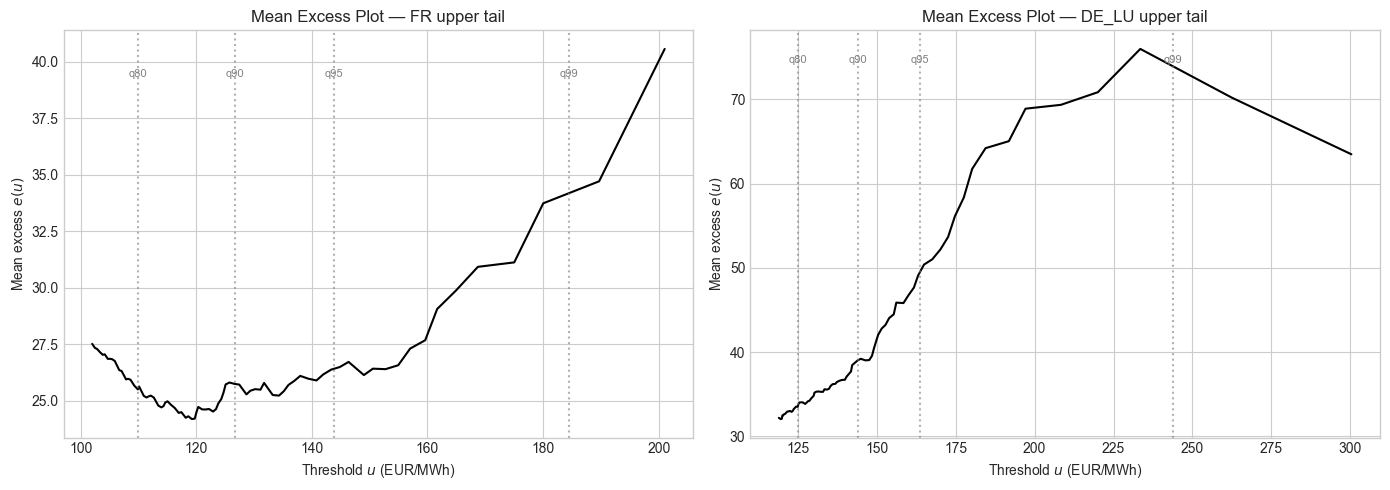
\includegraphics[width=\linewidth]{figures/mean-excess-upper.png}
    \caption{Mean Excess Plot for upper-tail exceedances in France and Germany.
             The approximately linear region identifies the range of viable thresholds.}
    \label{fig:mep_upper}
\end{figure}

\begin{figure}[H]
    \centering
    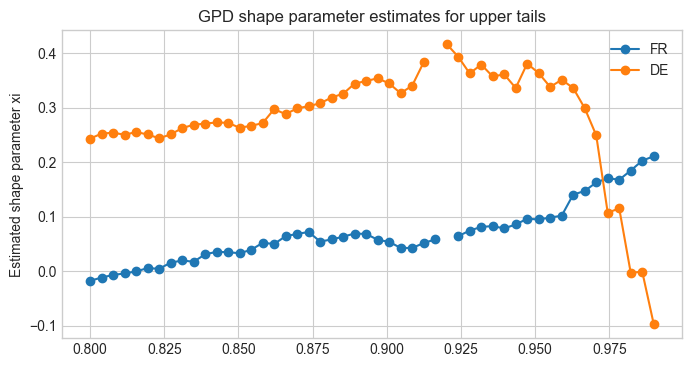
\includegraphics[width=0.75\linewidth]{figures/gpd-shape-upper.png}
    \caption{Estimated GPD shape parameter $\hat\xi$ as a function of the quantile
             threshold for the upper tail. The selected threshold $q = 0.93$ lies in
             a region of relative stability.}
    \label{fig:shape_upper}
\end{figure}

\begin{figure}[H]
    \centering
    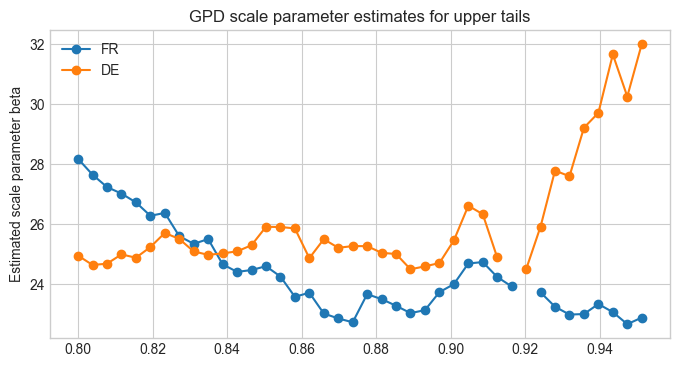
\includegraphics[width=0.75\linewidth]{figures/gpd-scale-upper.png}
    \caption{Estimated GPD scale parameter $\hat\beta$ as a function of the quantile
             threshold for the upper tail.}
    \label{fig:scale_upper}
\end{figure}

\begin{figure}[H]
    \centering
    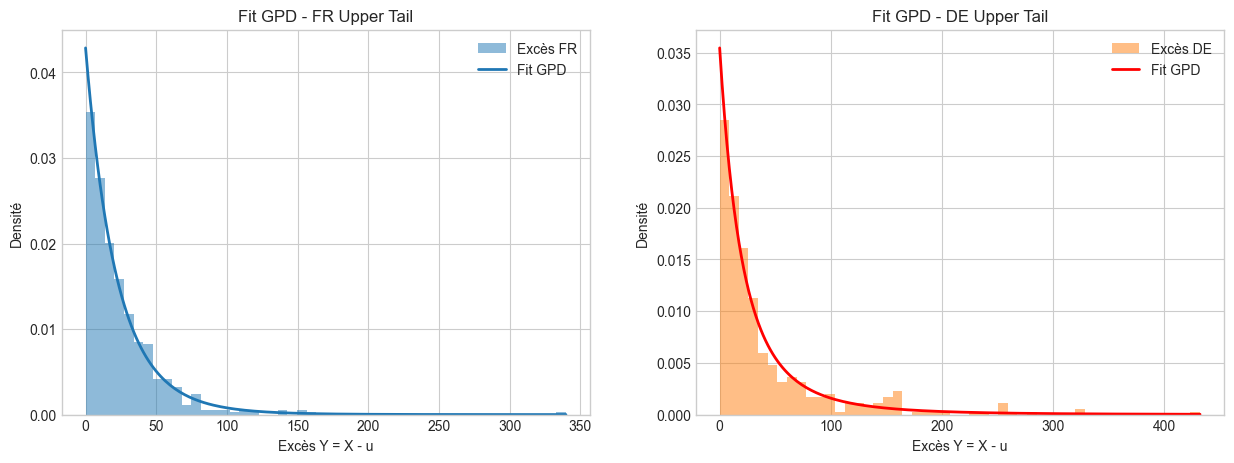
\includegraphics[width=\linewidth]{figures/gpd-fit-upper.png}
    \caption{Histogram of upper-tail exceedances and fitted GPD density for France
             (left) and Germany (right) at quantile threshold $q = 0.93$.}
    \label{fig:gpd_upper}
\end{figure}

\begin{figure}[H]
    \centering
    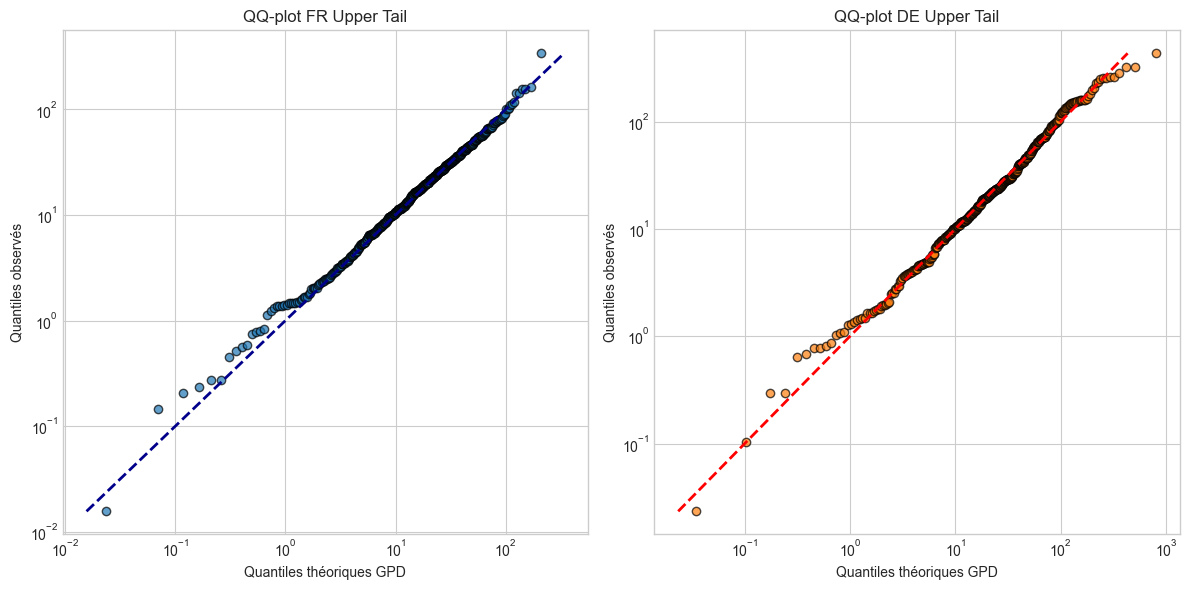
\includegraphics[width=\linewidth]{figures/qq-plot-upper.png}
    \caption{QQ-plot of the upper-tail exceedances against the fitted GPD quantiles
             for France (left) and Germany (right).}
    \label{fig:qq_upper}
\end{figure}

% ------------------------------------------------------------
\subsection{Lower Tail: Negative Prices}
\label{subsec:lower_tail}
% ------------------------------------------------------------

\paragraph{Threshold selection.}
The lower-tail analysis mirrors the upper-tail procedure. Figure~\ref{fig:mep_lower}
displays the lower-tail analogue of the Mean Excess Plot over a
grid of quantile thresholds $q \in [0.005, 0.25]$. The approximately linear region lies clearly to the right of zero
in both panels, which points to close to $u = 0$ as the natural threshold for the lower-tail analysis.

Figures~\ref{fig:shape_lower} and~\ref{fig:scale_lower} show the estimated shape and scale
parameters as a function of the lower quantile threshold. Stability is reached around
$q = 0.025$ for both France and Germany. This threshold is selected for the final
estimation and is reported in Table~\ref{tab:thresholds_lower}.

\begin{table}[H]
\centering
\caption{Selected thresholds and number of lower-tail exceedances at quantile $q = 0.025$.}
\label{tab:thresholds_lower}
\begin{tabular}{lcc}
\hline
Market & Threshold $u$ (EUR/MWh) & Number of exceedances $n_u$ \\
\hline
France     & $u_{\mathrm{FR}} = -1.67$ (2.5th pct.) & $169$ \\
Germany    & $u_{\mathrm{DE}} = -6.60$ (2.5th pct.) & $147$ \\
\hline
\end{tabular}
\end{table}


\paragraph{GPD fit.}
Figure~\ref{fig:gpd_lower} shows the histogram of lower-tail deficits and the fitted GPD
density for both markets. Figure~\ref{fig:qq_lower} provides the corresponding QQ-plots.
As with the upper tail, the fit is satisfactory across most of the distribution, with the
usual instability at the most extreme quantiles.

\begin{figure}[H]
    \centering
    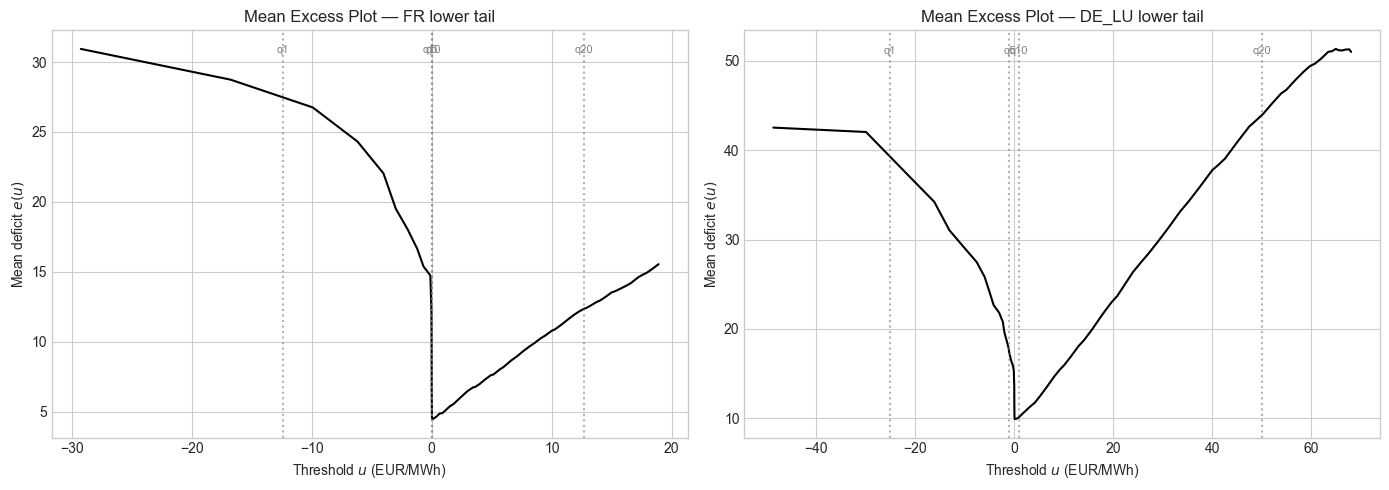
\includegraphics[width=\linewidth]{figures/mean-excess-lower.png}
    \caption{Mean Deficit Plot for lower-tail exceedances in France and Germany.
             The approximately linear region guides the threshold choice.}
    \label{fig:mep_lower}
\end{figure}

\begin{figure}[H]
    \centering
    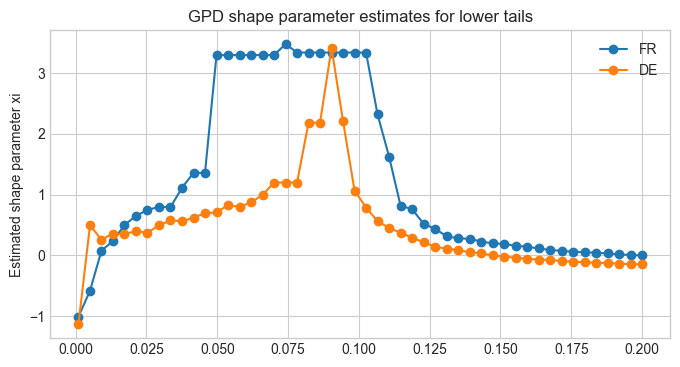
\includegraphics[width=0.75\linewidth]{figures/gpd-shape-lower.png}
    \caption{Estimated GPD shape parameter $\hat\xi$ as a function of the quantile
             threshold for the lower tail.}
    \label{fig:shape_lower}
\end{figure}

\begin{figure}[H]
    \centering
    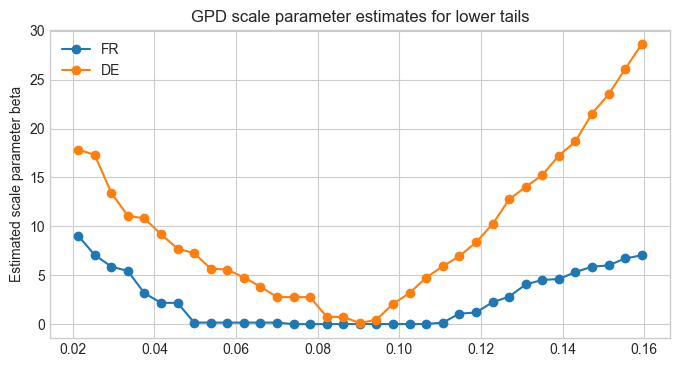
\includegraphics[width=0.75\linewidth]{figures/gpd-scale-lower.png}
    \caption{Estimated GPD scale parameter $\hat\beta$ as a function of the quantile
             threshold for the lower tail.}
    \label{fig:scale_lower}
\end{figure}

\begin{figure}[H]
    \centering
    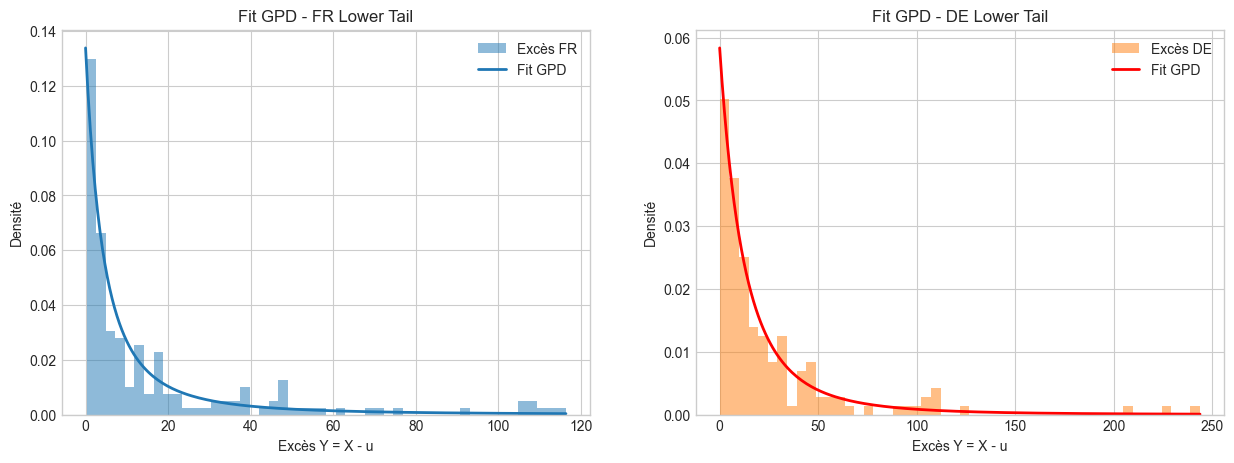
\includegraphics[width=\linewidth]{figures/gpd-fit-lower.png}
    \caption{Histogram of lower-tail deficits and fitted GPD density for France
             (left) and Germany (right) at quantile threshold $q = 0.025$.}
    \label{fig:gpd_lower}
\end{figure}

\begin{figure}[H]
    \centering
    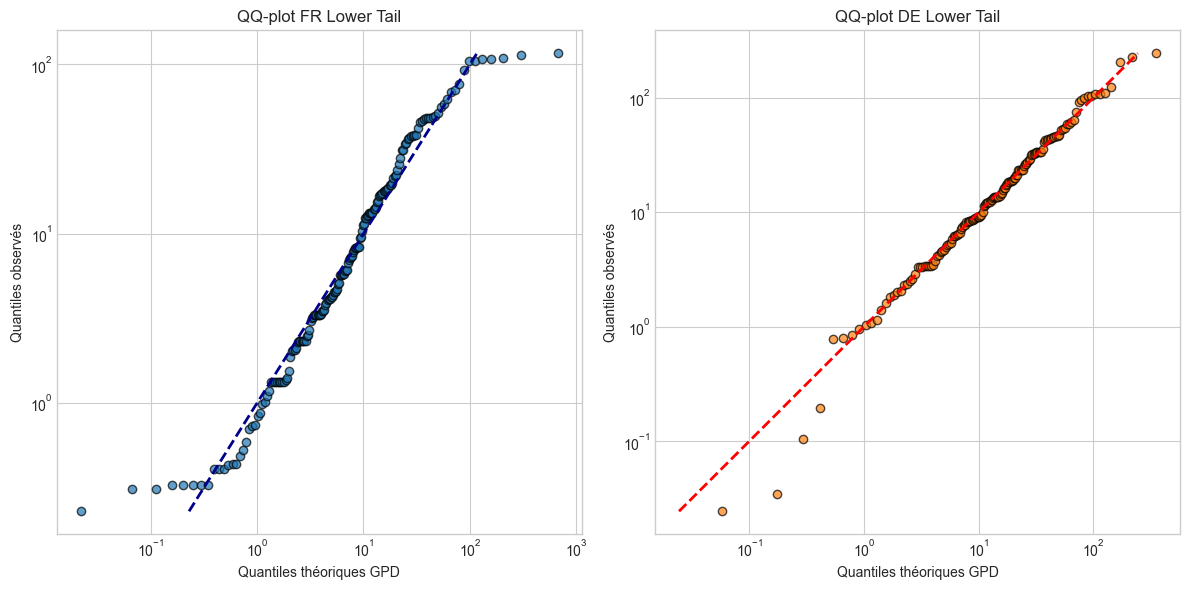
\includegraphics[width=\linewidth]{figures/qq-plot-lower.png}
    \caption{QQ-plot of the lower-tail deficits against the fitted GPD quantiles
             for France (left) and Germany (right).}
    \label{fig:qq_lower}
\end{figure}


% ------------------------------------------------------------
\subsection{Robustness: The Hill Estimator}
\label{subsec:hill}
% ------------------------------------------------------------

As an additional check on the GPD maximum-likelihood estimates, we compute the
\textbf{Hill estimator}, a semi-parametric estimator of the tail index valid in the
heavy-tailed (Fréchet) domain $\xi > 0$. For a sample $X_{(1)} \geq X_{(2)} \geq
\cdots \geq X_{(n)}$ of order statistics, the Hill estimator with $k$ upper-order
statistics is

\begin{equation}
    \hat\xi_H(k) = \frac{1}{k} \sum_{i=1}^{k} \log X_{(i)} - \log X_{(k+1)}.
    \label{eq:hill}
\end{equation}

The Hill plot traces $\hat\xi_H(k)$ as a function of $k$ and the optimal estimate is
read from the stable plateau of this curve. For the lower tail, the estimator is applied
to the reflected series $-X$. Figures~\ref{fig:hill_upper} and~\ref{fig:hill_lower} display
the Hill plots for the upper and lower tails respectively.

\begin{figure}[H]
    \centering
    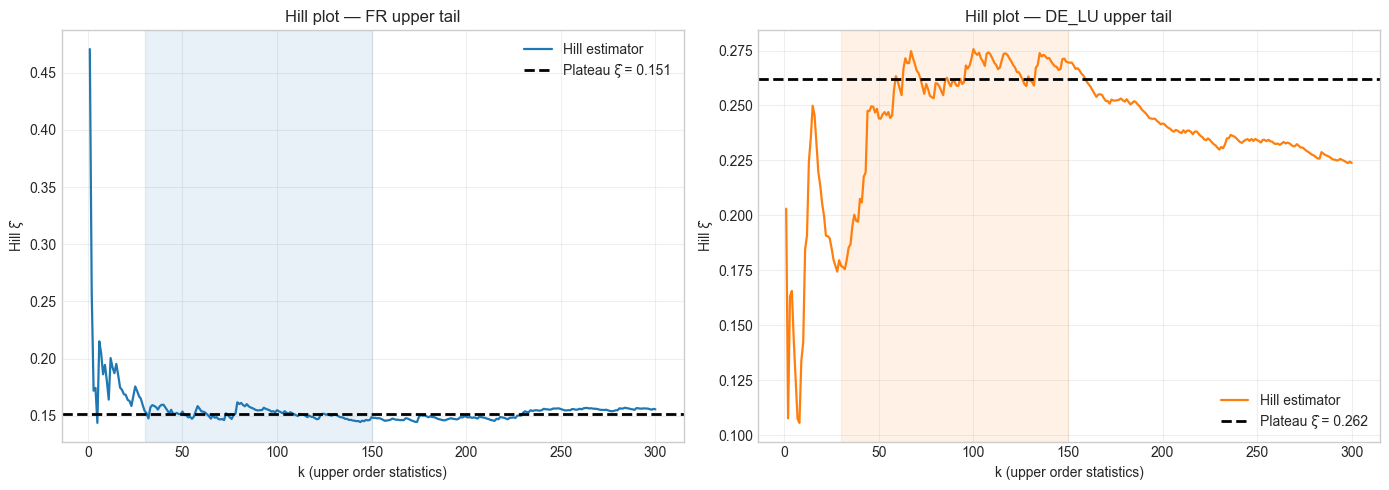
\includegraphics[width=\linewidth]{figures/hill-upper.png}
    \caption{Hill plots for the upper tail of French and German prices. The stable
             plateau in the range $k \in [30, 150]$ provides the Hill estimate.}
    \label{fig:hill_upper}
\end{figure}

\begin{figure}[H]
    \centering
    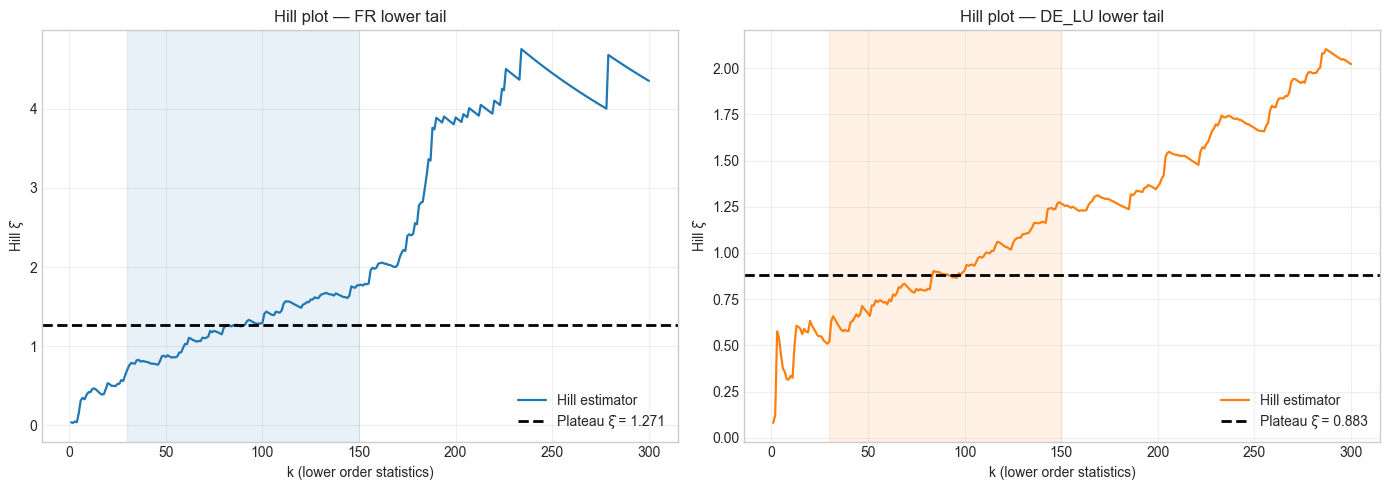
\includegraphics[width=\linewidth]{figures/hill-lower.png}
    \caption{Hill plots for the lower tail (reflected series) of French and German prices.}
    \label{fig:hill_lower}
\end{figure}

% ------------------------------------------------------------
\subsection{Summary of Tail Parameter Estimates}
\label{subsec:tail_summary}
% ------------------------------------------------------------

Table~\ref{tab:tail_params} consolidates the shape parameter estimates from both
methods for each market and each tail.

\begin{table}[H]
\centering
\caption{Estimated tail shape parameters $\hat\xi$ from GPD maximum likelihood
         and from the Hill estimator, for the upper and lower tails of the French
         and German day-ahead price series.}
\label{tab:tail_params}
\begin{tabular}{llcc}
\hline
Market & Tail  & $\hat\xi$ (GPD MLE) & $\hat\xi$ (Hill) \\
\hline
France  & Upper & $0.0735$  & $0.1514$ \\
Germany & Upper & $0.3601$  & $0.2621$ \\
France  & Lower & $0.7185$  & $1.2708$ \\
Germany & Lower & $0.3842$  & $0.8833$ \\
\hline
\end{tabular}
\end{table}


% ------------------------------------------------------------
\subsection{Interpretation}
\label{subsec:evt_interpretation}
% ------------------------------------------------------------

Several conclusions emerge from this analysis.

\paragraph{All tails are heavy.}
Every estimated shape parameter satisfies $\hat\xi > 0$, placing both markets
unambiguously in the Fréchet domain of attraction. This confirms that day-ahead
electricity prices exhibit power-law behaviour in both tails, which has direct consequences for risk
management and market design.

\paragraph{Strong asymmetry between upper and lower tails.}
A structural asymmetry emerges between the two directions of extreme events. For both
France and Germany, the lower tail is substantially heavier than the upper tail:

\[
    \hat\xi_{\mathrm{lower}} \gg \hat\xi_{\mathrm{upper}}.
\]

This finding is meaningful. Negative price episodes appear to generate
more extreme deviations relative to their threshold than positive price spikes. In other
words, when prices fall below zero, they can fall very far; the lower tail exhibits more
pronounced extremity than the upper tail.

\paragraph{Structural differences between France and Germany.}
Beyond the common heavy-tail finding, the two markets differ in their relative tail
behaviour. For the upper tail, Germany exhibits a heavier tail than France:

\[
    \hat\xi_{\mathrm{DE}}^{\mathrm{upper}} > \hat\xi_{\mathrm{FR}}^{\mathrm{upper}},
\]

indicating that, conditional on exceeding a selected threshold, very large positive price spikes 
tend to be more extreme in the German market. Conversely, for the lower tail, France appears to exhibit heavier extremes:

\[
    \hat\xi_{\mathrm{FR}}^{\mathrm{lower}} > \hat\xi_{\mathrm{DE}}^{\mathrm{lower}},
\]

suggesting that extreme negative price episodes are relatively more pronounced in France
once they materialise. These cross-country asymmetries motivate the regime-conditioned
copula analysis of Section~\ref{sec:copulas}.

\paragraph{Robustness of the EVT characterisation.}
Despite methodological differences (the Hill estimator focuses exclusively on the
most extreme observations, whereas the GPD fit incorporates a broader set of
threshold exceedances) both approaches deliver qualitatively consistent conclusions.
They agree on the presence of heavy tails, on the asymmetry between upper and lower
tails, and on the relative ordering of tail heaviness across the two markets. The
Hill estimates tend to be somewhat larger, as expected from the fact that this estimator
is sensitive to the very outermost observations and can be upward-biased in finite
samples. The GPD MLE is therefore our preferred point estimate, but the Hill comparison
serves as a useful robustness check.

\paragraph{Implications for the subsequent analyses.}
The EVT analysis characterises the marginal tail behaviour of each series independently.
It does not address whether extreme events occur jointly across markets or whether they
cluster in time. However, the presence of heavy tails has two direct implications for the
rest of the report. First, since linear correlation is blind to the dependence structure
in the tails, the heavy-tail finding strengthens the case for using copulas to study cross-market dependence. 
Second, since the tail shape parameters confirm that price spikes are not
isolated outliers but rather draw from heavy-tailed distributions, the temporal clustering 
of these events, studied through Hawkes processes in Section~\ref{sec:hawkes}, is a
natural follow-up question.
